\begin{problem}{\kcpccymktitle}
    {표준 입력}{표준 출력}
    {\kcpccymktime\,초}{\kcpccymkmemory\,MB}{}{\kcpccymkscore}
    
    $ x $축, $ y $축으로 이루어진 평면 상에 직사각형들이 있다. 민성이는 지금부터 엄청나게 거대한 프린터기를 사용하여 이 평면 상의 직사각형들을 색칠할 것이다. 이 직사각형들의 모든 변은 $ x $축 또는 $ y $축에 평행하다.
    
    민성이에게는 3가지 색상 - 시안, 노랑, 그리고 자홍색의 잉크가 있다. 어떤 직사각형 위에는 시안색을 칠하고, 어떤 직사각형 위에는 노랑색, 또 다른 어떤 직사각형 위에는 자홍색을 칠할 수 있다.
    
    어떤 경우에는 서로 다른 2개 이상의 직사각형의 영역이 겹쳐있어, 민성이가 가지고 있는 3가지 잉크의 색깔이 아닌 다른 색깔의 영역이 나타날 수 있다. 다음 그림은 시안, 노랑, 자홍색을 섞었을 때 나타날 수 있는 색깔들이다.
    
    \begin{figure}[h]
        \centering
        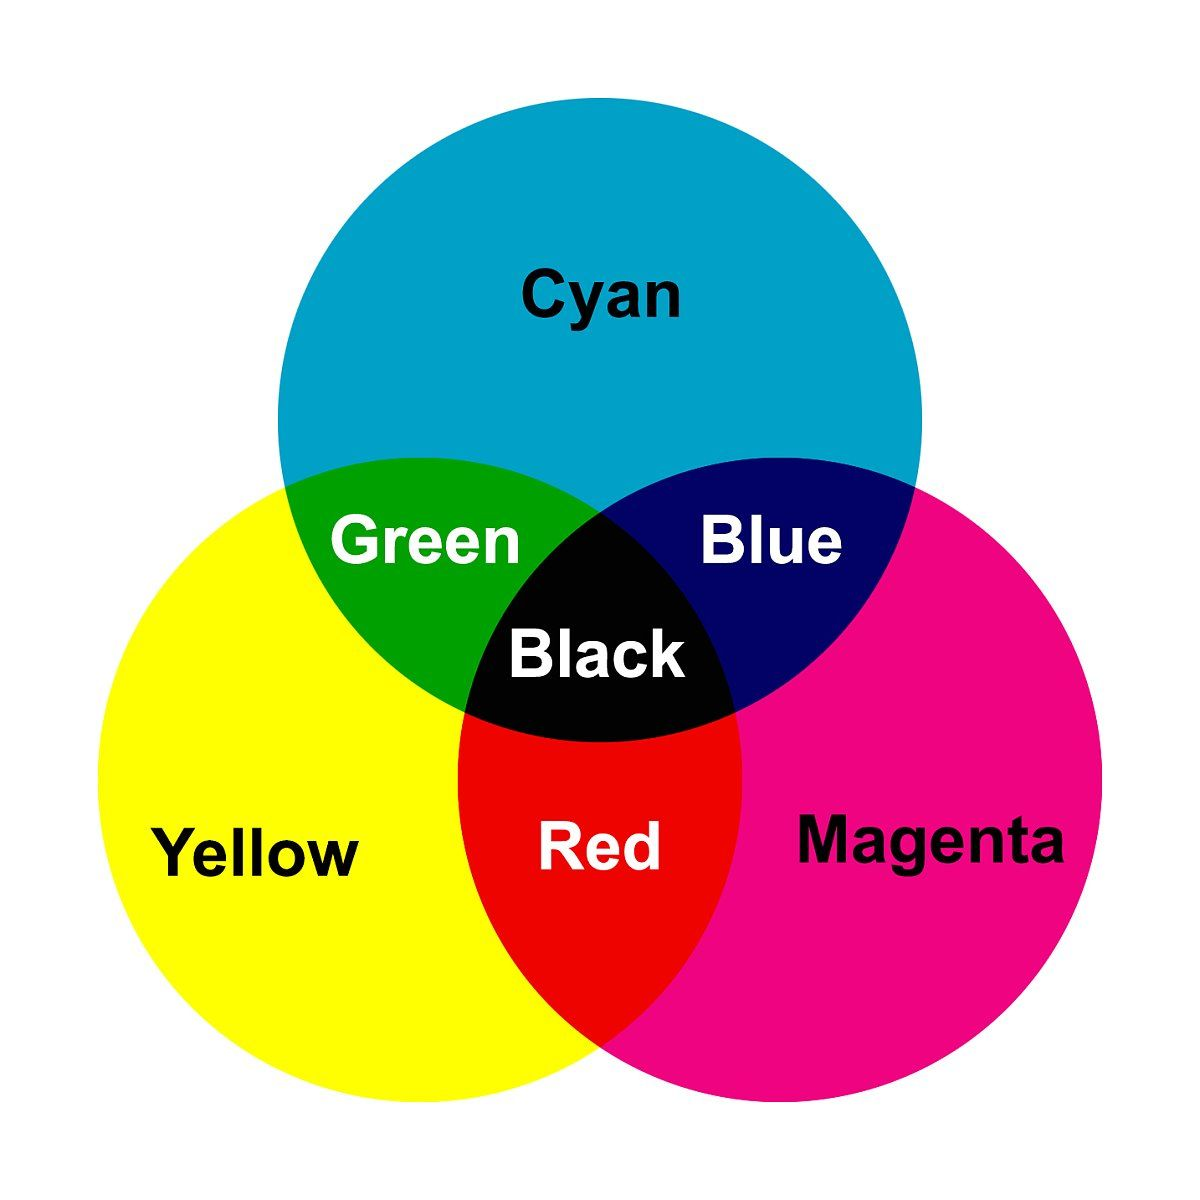
\includegraphics[width=0.4\textwidth]{./problems/cymk.jpeg}
    \end{figure}
    
    즉 빨간색은 자홍색과 노란색이, 초록색은 노란색과 시안색이, 파란색은 자홍색과 시안색이, 검은색은 자홍색과 노란색과 시안색이 동일한 비율로 섞인 색이다.
    
    단, 민성이는 잉크를 아끼기 위해 한번 어떤 색깔로 색칠한 곳은 이후에 동일한 색깔의 겹치는 직사각형 영역이 나타나더라도 한번만 칠하기로 했다. 예를 들어서, (0, 0)부터 (2, 2)까지의 영역에 민성이가 노란색을 칠한 후 다시 (1, 1)부터 (3, 3)까지 노란색을 칠해야 하는 상황이 왔다면, (1, 1)부터 (2, 2)까지는 이미 노란색이 색칠되어 있으므로 다시 노란색을 덧칠하지 않는다. 이렇게 되면 3원색이 섞이는 비율이 항상 동일하기 때문에, 민성이가 잉크를 아끼게 됨과 동시에 위 그림에 나오지 않은 색깔이 등장할 일도 없어지게 된다.
    
    당신은 서로 다른 색깔로 칠할 직사각형들이 주어졌을 때, 민성이가 주어진 색깔대로 모두 칠한 후 각 색깔별 영역의 넓이를 민성이가 일일이 색칠하기 전에 미리 구하고자 한다.
    
    \InputFile
    첫 번째 줄에 입력받을 직사각형의 개수 $ N $이 주어진다. $ (1 \leq N \leq 25,000) $
    
    두 번째 줄부터 $ N $개의 줄에 걸쳐 각 직사각형의 정보를 나타내는 정수 $ x_1,\ y_1,\ x_2,\ y_2 $와 문자 $ c $가 공백으로 구분되어 주어진다. $ (-10^8 \leq x_1 < x_2 \leq 10^8,\ -10^8 \leq y_1 < y_2 \leq 10^8) $
    
    이는 해당하는 직사각형이 $ (x_1, y_1),\ (x_1, y_2),\ (x_2, y_2),\ (x_2, y_1) $를 꼭짓점으로 가지고 $ c $에 해당하는 색깔로 칠해짐을 의미한다.
    
    모든 $ c $는 1글자짜리 문자로, \verb|"C"|(시안), \verb|"M"|(자홍), \verb|"Y"|(노랑) 중 하나이다.
    
    \OutputFile
    첫 번째 줄에 일곱 개의 정수 $ S_c,\ S_m,\ S_y,\ S_r,\ S_g,\ S_b,\ S_k $을 공백으로 구분하여 출력한다. 각각 시안색 영역의 넓이, 자홍색 영역의 넓이, 노란색 영역의 넓이, 빨간색 영역의 넓이, 초록색 영역의 넓이, 파란색 영역의 넓이, 그리고 검정색 영역의 넓이를 의미한다.
    
    (0,0), (1,0), (1,1), (0,1)을 꼭짓점으로 가지는 직사각형의 넓이는 1이다.
    
    
    \SubtaskWithScore{\kcpccymksmallscore}
    $ 1 \leq N \leq 500 , -10^4 \leq x_1 < x_2 \leq 10^4, -10^4 \leq y_1 < y_2 \leq 10^4 $ 을 만족한다.
    
    \SubtaskWithScore{\kcpccymklargescore}
    문제 입력에서 주어진 조건 외에 추가적인 조건이 없다.

    \Examples
    
    \begin{example}
        \exmp{
            4
            0 0 3 3 C
            1 1 4 4 M
            2 -1 5 2 Y
            5 4 6 5 C
        }{%
            5 4 6 1 1 3 1
        }%
    \end{example}
    
    \Explanation
    다음 그림은 첫 번째 예제를 그림으로 표현한 것이다.
    
    \begin{figure}[h]
        \centering
        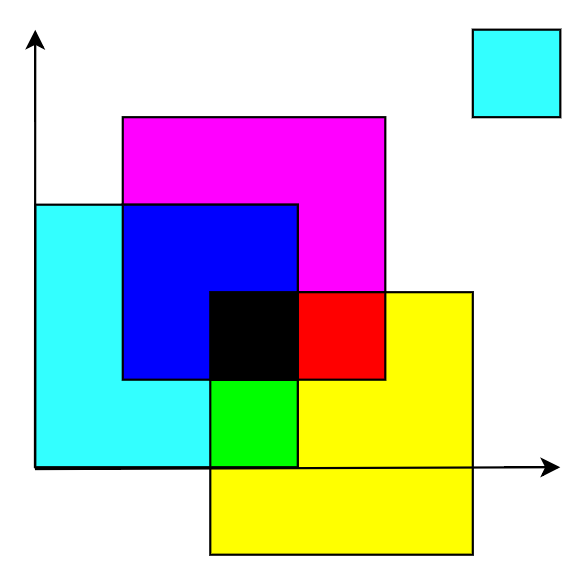
\includegraphics[width=0.4\textwidth]{./problems/cymk-ex.png}
    \end{figure}
    
\end{problem}

